\documentclass[a4paper,11pt]{article}

\usepackage[T1]{fontenc}
\usepackage[slovene]{babel}
\usepackage{graphicx}

\title{Pregled obstoječih rešitev\\
Spletna stran za avtoservis}
\author{Luka Jesenšek}
\date{25.\ november 2026}

\begin{document}

\maketitle
\tableofcontents
\newpage

%------------------------------------------------------------
\section{Uvod}

Namen projekta je izdelava spletne strani za avtoservis, ki bo uporabnikom omogočala pregled storitev, cenika in kontaktnih podatkov ter spletno naročanje na servis. S spletno stranjo želim uporabnikom olajšati dostop do informacij in omogočiti naročanje brez telefonskega klica.

%NFS
\section{Pregled obstoječih rešitev}

\subsection{NFS Avtoservis}

\subsubsection{Opis}

NFS Avtoservis je podjetje iz Maribora, ki ponuja servisiranje vozil, vulkanizerstvo in čiščenje vozil. Na spletni strani so predstavljene storitve, cenik in kontaktni podatki podjetja \cite{nfs}.

\subsubsection{Ključne funkcionalnosti}

\begin{itemize}
    \item Pregled servisnih storitev.
    \item Pregled cenika storitev.
    \item Pregled ponudb.
    \item Prikaz kontaktov.
    \item Prikaz lokacije servisa.
\end{itemize}

\subsubsection{Prednosti}

\begin{itemize}
    \item Rrazvrščene storitve.
    \item Prikazane cene storitev.
    \item Enostaven dostop do kontaktnih podatkov.
    \item Preprosta navigacija
\end{itemize}

\subsubsection{Slabosti}

\begin{itemize}
    \item Nii obrazca za naročanje.
    \item Ni prikaza prostih terminov.
    \item Za dogovor o terminu je potrebeno klicati.
\end{itemize}

\begin{figure}[h]
    \centering
    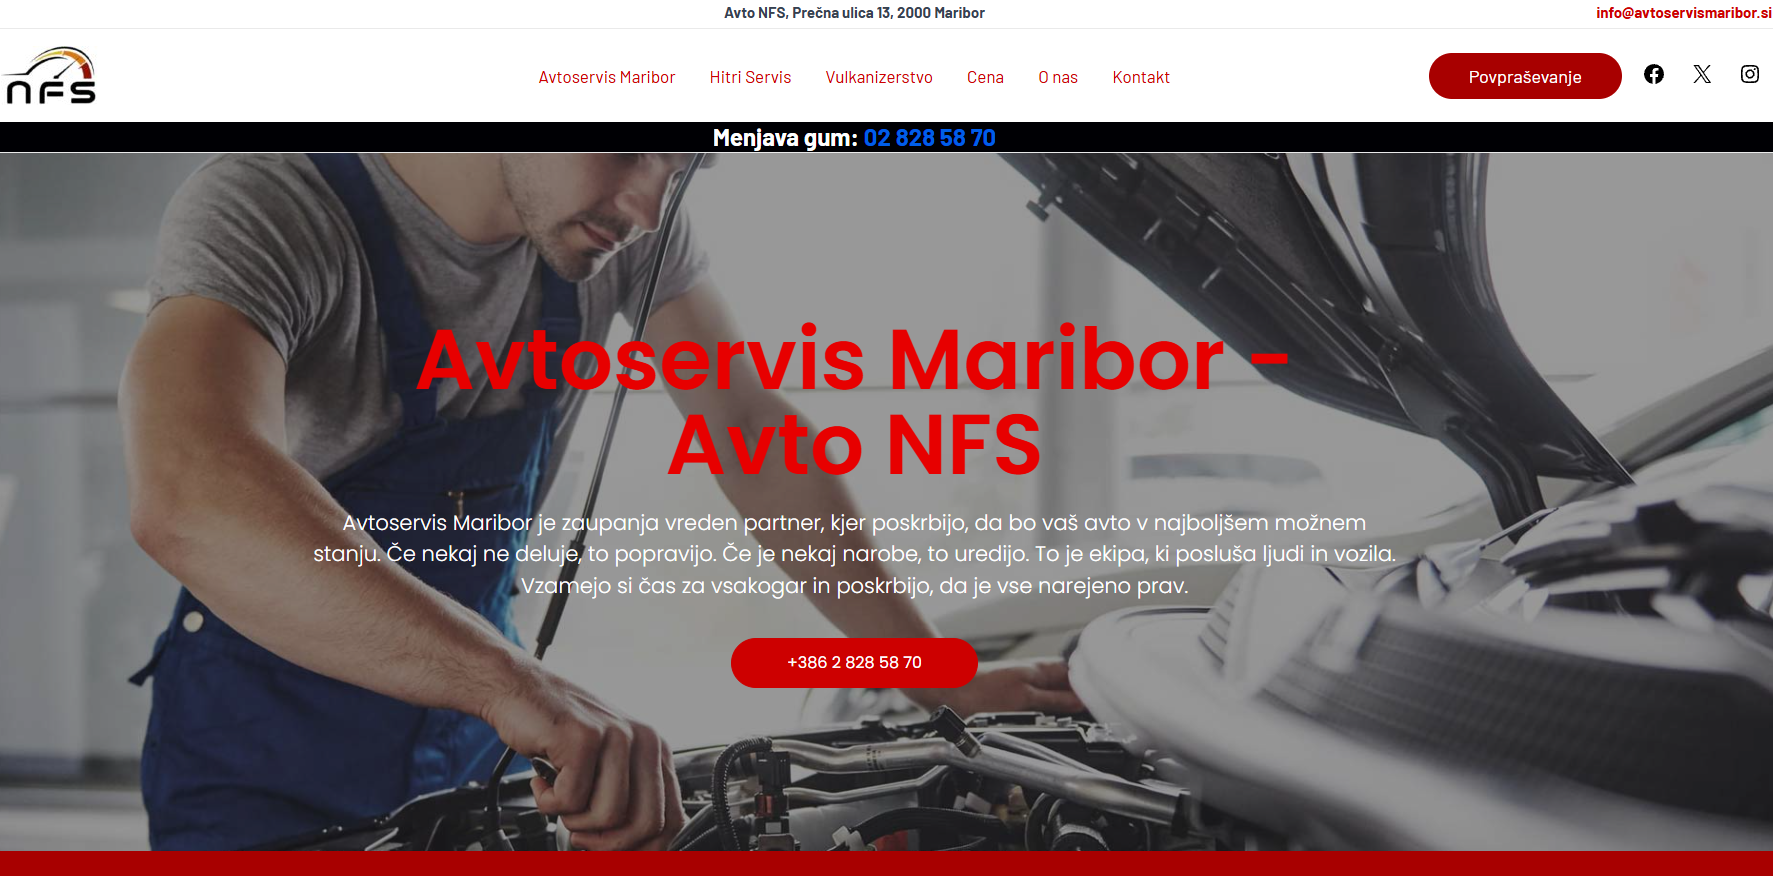
\includegraphics[width=\textwidth]{nfs.png}
    \caption{Spletna stran NFS Avtoservis.}
    \label{fig:nfs}
\end{figure}

\clearpage

%AMZS
\subsection{AMZS}

\subsubsection{Opis}

AMZS je organizacija, ki ponuja različne storitve na področju avtomobilizma. Med njimi je tudi servisiranje vozil. Spletna stran omogoča tudi prijavo na servis \cite{amzs}.

\subsubsection{Ključne funkcionalnosti}

\begin{itemize}
    \item Pregled servisnih storitev.
    \item Spletno naročanje na servis.
    \item Pregled lokacij servisnih centrov.
    \item Pregled delovnega časa.
    \item Pregled ponudb.
\end{itemize}

\subsubsection{Prednosti}

\begin{itemize}
    \item Možnost spletnega naročanja na servis.
    \item Opisi posameznih storitev.
    \item Info. o različnih servisnih centrih.
\end{itemize}

\subsubsection{Slabosti}

\begin{itemize}
    \item Veliko število kategorij in podstrani.
    \item Obsežna navigacija.
    \item Veliko informacij, ki ni povezana s servisiranjem vozil.
\end{itemize}

\begin{figure}[h]
    \centering
    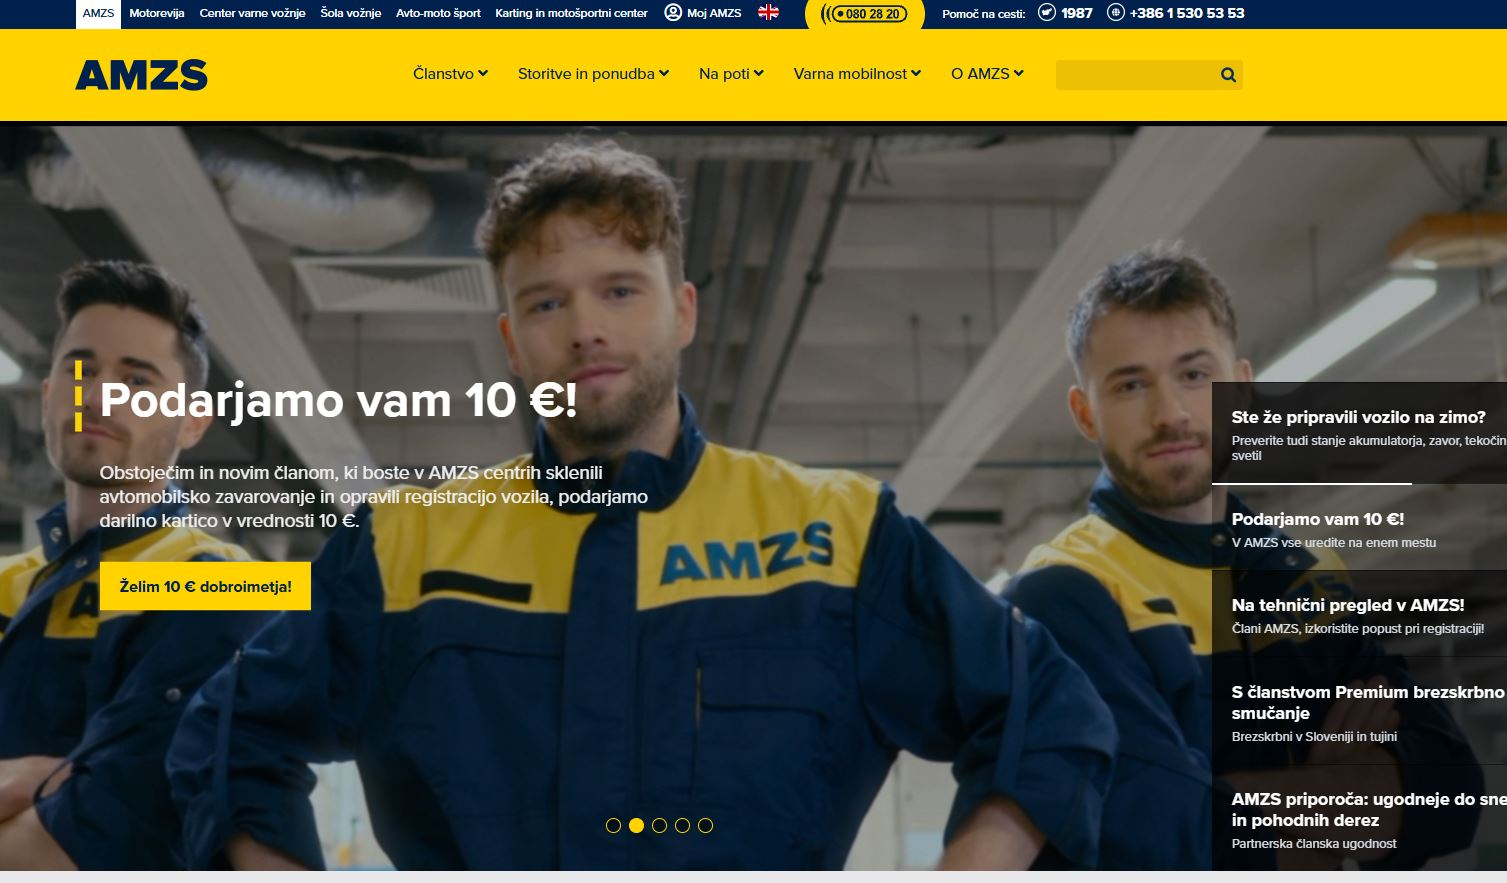
\includegraphics[width=\textwidth]{amzs.png}
    \caption{Spletna stran AMZS za naročanje na servis.}
    \label{fig:amzs}
\end{figure}

\clearpage

%CARFIX
\subsection{CAR FIX}

\subsubsection{Opis}

CAR FIX je ponudnik servisnih storitev za vozila. Podjetje ponuja redne servise, menjavo pnevmatik, vzdrževanje... Spletna stran omogoča pregled cen, spletno naročanje in oddajo povpraševanja. \cite{carfix}.

\subsubsection{Ključne funkcionalnosti}

\begin{itemize}
    \item Pregled servisnih storitev.
    \item Pregled cen posameznih storitev.
    \item Spletno naročanje na servis.
    \item Oddaja spletnega povpraševanja.
    \item Pregled lokacij poslovalnic.
\end{itemize}

\subsubsection{Prednosti}

\begin{itemize}
    \item Možnost spletnega naročanja.
    \item Predstavljene servisne storitve.
    \item Razdelitev cen glede na vrsto vozila.
    \item Možnost oddaje povpraševanja.
\end{itemize}

\subsubsection{Slabosti}

\begin{itemize}
    \item Veliko besedila na posamezni strani.
    \item Dolgo pomikanje po strani.
    \item Nekatere cene popravil niso določene vnaprej.
\end{itemize}

\begin{figure}[h]
    \centering
    
\includegraphics[width=\textwidth]{carfix.png}
    \caption{Spletna stran CAR FIX.}
    \label{fig:carfix}
\end{figure}

\clearpage

%------------------------------------------------------------
\section{Zaključek}

Pri izdelavi svoje spletne strani bom od NFS Avtoservisa prevzel način prikaza storitev in cenika. Od AMZS bom prevzel idejo spletnega naročanja, od CAR FIX pa način predstavitve posameznih servisnih storitev. Moja spletna stran bo imela preprosto navigacijo, pregleden cenik in obrazec za naročanje na servis. S tem želim omogočiti hitrejši dostop do informacij in enostavnejše naročanje na servis.

%Literatura
\begin{thebibliography}{9}

\bibitem{nfs}
NFS Avtoservis,\\
https://avtoservismaribor.si/

\bibitem{amzs}
AMZS, Naročilo na servis,\\
https://www.amzs.si/storitve/prijava-na-servis

\bibitem{carfix}
CAR FIX,\\
https://www.carfix.si/

\end{thebibliography}

\end{document}